\subsubsubsubsection{Street builder}
\begin{figure}[h]
\centering
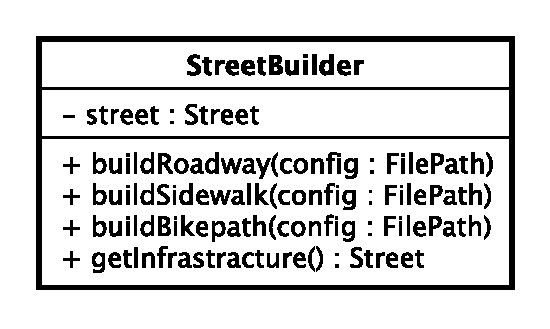
\includegraphics[scale=0.6,keepaspectratio]{images/solution/app/backend/street_builder.eps}
\caption{\pReactiveBuild::StreetBuilder}
\label{fig:sd-app-street_builder}
\end{figure}
\FloatBarrier
\begin{itemize}
  \item \textbf{\descr} \\
    It represents the builder of street entities.
  \item \textbf{\attrs}
  \begin{itemize}
    \item \texttt{street: Street} \\
The street which the builder incrementally constructs.
  \end{itemize}
  \item \textbf{\ops}
  \begin{itemize} 
    \item[+] \texttt{buildRoadway()} \\
Builds a roadway using \texttt{RoadwayFactory}.
    \item[+] \texttt{buildSidewalk()} \\
Builds a sidewalk using \texttt{SidewalkFactory}.
    \item[+] \texttt{buildBikepath()} \\
Builds a bikepath using \texttt{BikepathFactory}.
    \item[+] \texttt{getStreet() : Street} \\
Returns the street.
  \end{itemize}
\end{itemize}
